\chapter{Cortafuegos: Conceptos te\'oricos}
\section{Introducci\'on}
Seg\'un \cite{kn:firefaq}, un {\it firewall} o cortafuegos es un sistema o 
grupo de sistemas que hace cumplir una pol\'{\i}tica de control de acceso
entre dos redes. De una forma m\'as clara, podemos definir un cortafuegos como 
cualquier sistema (desde un simple {\it router} hasta varias redes en serie) 
utilizado para separar -- en cuanto a seguridad se refiere --
una m\'aquina o subred del resto, protegi\'endola as\'{\i} de servicios y 
protocolos que desde el exterior puedan suponer una amenaza a la seguridad. El
espacio protegido, denominado {\bf per\'{\i}metro de seguridad}, suele ser 
propiedad de la misma organizaci\'on, y la protecci\'on se realiza contra una 
red externa, no confiable, llamada {\bf zona de riesgo}.\\
\\Evidentemente la forma de aislamiento m\'as efectiva para cualquier 
pol\'{\i}tica de seguridad consiste en el aislamiento f\'{\i}sico, es decir, no
tener conectada la m\'aquina o la subred a otros equipos o a Internet (figura
\ref{lanwan} (a)). Sin embargo, en la mayor\'{\i}a de organizaciones --
especialmente en las de I+D -- los usuarios
necesitan compartir informaci\'on con otras personas situadas en muchas 
ocasiones a miles de kil\'ometros de distancia, con lo que no es posible un 
aislamiento total. El punto opuesto consistir\'{\i}a en una conectividad 
completa con la red (figura \ref{lanwan} (b)), lo que desde el punto de vista 
de la seguridad es muy
problem\'atico: cualquiera, desde cualquier parte del mundo, puede 
potencialmente tener acceso a nuestros recursos. Un t\'ermino medio entre ambas 
aproximaciones consiste en implementar cierta separaci\'on l\'ogica mediante un 
cortafuegos (figura \ref{lanwan} (c)).\\
\begin{figure}
\begin{center}
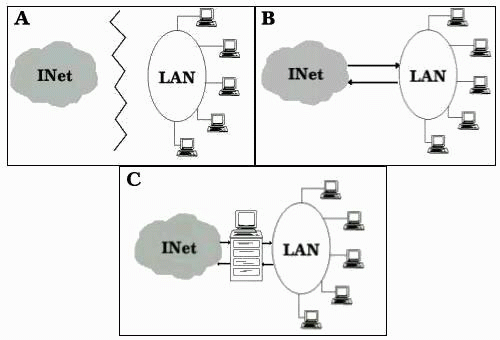
\includegraphics[width=\textwidth]{fw.png}
\caption{(a) Aislamiento. (b) Conexi\'on total. (c) {\it Firewall} entre la
zona de riesgo y el per\'{\i}metro de seguridad.}
\label{lanwan}
\end{center}
\end{figure}
\\Antes de hablar de cortafuegos es casi obligatorio dar una serie
de definiciones de partes o caracter\'{\i}sticas de funcionamiento de un {\it
firewall}; por m\'aquina o {\it host} {\bf basti\'on} (tambi\'en se denominan
{\bf gates}) se conoce a un sistema especialmente asegurado, pero en principio
vulnerable a todo tipo de ataques por estar abierto
a Internet, que tiene como funci\'on ser el punto de contacto de los usuarios
de la red interna de una organizaci\'on con otro tipo de redes. El {\it host}
basti\'on filtra tr\'afico de entrada y salida, y tambi\'en esconde la 
configuraci\'on de la red hacia fuera.\\
\\Por {\bf filtrado de paquetes} entendemos la acci\'on de denegar o permitir
el flujo de tramas entre dos redes (por ejemplo la interna, protegida con el
{\it firewall}, y el resto de Internet) de acuerdo a unas normas predefinidas;
aunque el filtro m\'as elemental puede ser un simple {\it router}, trabajando 
en el nivel de red del protocolo OSI, esta actividad puede realizarse 
adem\'as en un puente o en una m\'aquina individual. El filtrado tambi\'en se 
conoce como {\it screening}, y a los dispositivos que lo implementan se les
denomina {\bf chokes}; el {\it choke} puede ser la m\'aquina basti\'on o un
elemento diferente.\\
\\Un {\bf proxy} es un programa (trabajando en el nivel de aplicaci\'on de OSI)
que permite o niega el acceso a una aplicaci\'on determinada entre dos redes. 
Los clientes {\it proxy} se comunican s\'olo con los servidores {\it proxy}, 
que autorizan las peticiones y las env\'{\i}an a los servidores reales, o las
deniegan y las devuelven a quien las solicit\'o.\\
\\F\'{\i}sicamente, en casi todos los cortafuegos existen al menos un {\it 
choke} y una m\'aquina basti\'on, aunque tambi\'en se considera {\it firewall} 
a un simple {\it router} filtrando paquetes, es decir, actuando como {\it 
choke}; desde el punto de vista l\'ogico, en el cortafuegos suelen existir 
servidores {\it proxy} para las aplicaciones que han de atravesar el sistema, y
que se situan habitualmente en el {\it host} basti\'on. Tambi\'en se implementa
en el {\it choke} un mecanismo de filtrado de paquetes, y en alguno de los
dos elementos se suele situar otro mecanismo para poder monitorizar y detectar 
la actividad sospechosa.\\
\\En este cap\'{\i}tulo hablaremos de los tipos de cortafuegos m\'as 
habituales y de sus caracter\'{\i}sticas, as\'{\i} como de las posibles 
pol\'{\i}ticas de seguridad que pueden implementar; en el siguiente 
comentaremos aspectos de algunos de los cortafuegos m\'as utilizados hoy en 
d\'{\i}a, como {\it FireWall-1} o Cisco PIX Firewall. Los {\it firewalls} son 
cada vez m\'as
necesarios en nuestras redes, pero todos los expertos recomiendan que no se usen
{\bf en lugar de} otras herramientas, sino {\bf junto a} ellas; cualquier 
cortafuegos, desde el m\'as simple al m\'as avanzado, presenta dos 
grav\'{\i}simos problemas de seguridad: por un lado, centralizan todas las 
medidas en un \'unico sistema, de forma que si \'este se ve comprometido y 
el resto de nuestra red no est\'a lo suficientemente protegido el atacante 
consigue amenazar a toda la subred simplemente poniendo en jaque a una 
m\'aquina. El segundo problema, relacionado con \'este, es la falsa sensaci\'on
de seguridad que un cortafuegos proporciona: generalmente un administrador que
no disponga de un {\it firewall} va a preocuparse de la integridad de todas y
cada una de sus m\'aquinas, pero en el momento en que instala el cortafuegos
y lo configura asume que toda su red es segura, por lo que se suele descuidar
enormemente la seguridad de los equipos de la red interna. Esto, como acabamos
de comentar, es un grave error, ya que en el momento que un pirata acceda a
nuestro cortafuegos -- recordemos que es un sistema muy expuesto a ataques
externos -- autom\'aticamente va a tener la posibilidad de controlar toda 
nuestra red.\\
\\Adem\'as -- esto ya no es un problema de los {\it firewalls} sino
algo de sentido com\'un --, un cortafuegos evidentemente no protege contra 
ataques que no pasan por \'el: esto incluye todo tipo de ataques internos dentro
del per\'{\i}metro de seguridad, pero tambi\'en otros factores que {\it a
priori} no deber\'{\i}an suponer un problema. El t\'{\i}pico ejemplo de estos
\'ultimos son los usuarios que instalan sin permiso, sin conocimiento del 
administrador de la red, y muchas veces sin pensar en sus consecuencias, un
simple {\it modem} en sus PCs o estaciones de trabajo; esto, tan habitual en
muchas organizaciones, supone la violaci\'on y la ruptura total del 
per\'{\i}metro de seguridad, ya que posibilita accesos a la red no controlados
por el cortafuegos. Otro problema de sentido com\'un es la reconfiguraci\'on
de los sistemas al pasarlos de una zona a otra con diferente nivel de seguridad,
por ejemplo al mover un equipo que se encuentra en el \'area protegida a la
DMZ (veremos m\'as adelante lo que estas siglas significan); este acto -- que
en ocasiones no implica ni tan siquiera el movimiento f\'{\i}sico del equipo, 
sino simplemente conectarlo en una toma de red diferente -- puede ocasionar
graves problemas de seguridad en nuestra organizaci\'on, por lo que cada vez que
un cambio de este estilo se produzca no s\'olo es necesaria la reconfiguraci\'on
del sistema, sino la revisi\'on de todas las pol\'{\i}ticas de seguridad
aplicadas a esa m\'aquina (\cite{kn:mel97}).
\section{Caracter\'{\i}sticas de dise\~no}
Existen tres decisiones b\'asicas en el dise\~no o la configuraci\'on de un 
cortafuegos (\cite{kn:firefaq}); la primera de ellas, la m\'as importante, hace 
referencia a la pol\'{\i}tica de seguridad de la organizaci\'on propietaria del 
{\it firewall}: evidentemente, la configuraci\'on y el nivel de seguridad 
potencial ser\'a distinto en una empresa que utilice un cortafuegos para 
bloquear todo el tr\'afico externo hacia el dominio de su propiedad (excepto, 
quiz\'as, las consultas a su p\'agina
{\it web}) frente a otra donde s\'olo se intente evitar que los usuarios 
internos pierdan el tiempo en la red, bloqueando por ejemplo todos los servicios
de salida al exterior excepto el correo electr\'onico. Sobre esta decisi\'on
influyen, aparte de motivos de seguridad, motivos administrativos de cada
organismo.\\
\\La segunda decisi\'on de dise\~no a tener en cuenta es el nivel de 
monitorizaci\'on, redundancia y control deseado en la organizaci\'on; una vez
definida la pol\'{\i}tica a seguir, hay que definir c\'omo implementarla en el
cortafuegos indicando b\'asicamente qu\'e se va a permitir y qu\'e se va a 
denegar. Para esto existen dos aproximaciones generales: o bien se adopta una
postura restrictiva (denegamos todo lo que expl\'{\i}citamente no se permita) o
bien una permisiva (permitimos todo excepto lo expl\'{\i}citamente negado);
evidentemente es la primera la m\'as recomendable de cara a la seguridad, pero
no siempre es aplicable debido a factores no t\'ecnicos sino humanos (esto
es, los usuarios y sus protestas por no poder ejecutar tal o cual aplicaci\'on
a trav\'es del {\it firewall}).\\
\\Por \'ultimo, la tercera decisi\'on a la hora de instalar un sistema de 
cortafuegos es
meramente econ\'omica: en funci\'on del valor estimado de lo que deseemos 
proteger, debemos gastar m\'as o menos dinero, o no gastar nada. Un {\it 
firewall} puede no entra\~nar gastos extras para la organizaci\'on, o suponer
un desembolso de varios millones de pesetas: seguramente un departamento o 
laboratorio con pocos equipos en su interior puede utilizar un PC con Linux,
Solaris o FreeBSD a modo de cortafuegos, sin gastarse nada en \'el (excepto
unas horas de trabajo y unas tazas de caf\'e), pero esta aproximaci\'on 
evidentemente no funciona cuando el sistema a proteger es una red de tama\~no
considerable; en este caso se pueden utilizar sistemas 
propietarios, que suelen ser caros, o aprovechar los {\it routers} de salida
de la red, algo m\'as barato pero que requiere m\'as tiempo de configuraci\'on
que los cortafuegos sobre Unix en PC de los que hemos hablado antes. De 
cualquier forma, no es recomendable a la hora de evaluar el dinero a invertir
en el {\it firewall} fijarse s\'olo en el coste de su instalaci\'on y puesta
a punto, sino tambi\'en en el de su mantenimiento.\\
\\Estas decisiones, aunque concernientes al dise\~no, eran b\'asicamente 
pol\'{\i}ticas; la primera decisi\'on t\'ecnica a la que nos vamos a enfrentar
a la hora de instalar un cortafuegos es elemental: >d\'onde lo situamos para
que cumpla eficientemente su cometido? Evidentemente, si aprovechamos como 
cortafuegos un equipo ya existente en la red, por ejemplo un {\it router}, no
tenemos muchas posibilidades de elecci\'on: con toda seguridad hemos de dejarlo
donde ya est\'a; si por el contrario utilizamos una m\'aquina Unix con un
cortafuegos implementado en ella, tenemos varias posibilidades para situarla
con respecto a la red externa y a la interna. Sin importar donde situemos al
sistema hemos de recordar siempre que los equipos que queden fuera del 
cortafuegos, en la zona de riesgo, ser\'an igual de vulnerables que antes de
instalar el {\it firewall}; por eso es posible que si por obligaci\'on hemos 
tenido que instalar un cortafuegos en un punto que no protege completamente
nuestra red, pensemos en a\~nadir cortafuegos internos dentro de la misma,
aumentando as\'{\i} la seguridad de las partes m\'as importantes.\\
\\Una vez que hemos decidido d\'onde situar nuestro cortafuegos se debe elegir
qu\'e elemento o elementos f\'{\i}sicos utilizar como basti\'on; para tomar
esta decisi\'on existen dos principios b\'asicos (\cite{kn:bre95}): m\'{\i}nima
complejidad y m\'axima seguridad. Cuanto m\'as simple sea el {\it host} 
basti\'on, cuanto menos servicios ofrezca, m\'as f\'acil ser\'a su 
mantenimiento y por tanto mayor su seguridad; mantener esta m\'aquina 
especialmente asegurada es algo vital para que el cortafuegos funcione 
correctamente, ya que va a soportar por s\'{\i} sola todos los ataques que se 
efectuen contra nuestra red al ser elemento m\'as accesible de \'esta. Si la
seguridad de la m\'aquina basti\'on se ve comprometida, la amenaza se traslada
inmediantamente a todos los equipos dentro del per\'{\i}metro de seguridad.
Suele ser una buena opci\'on elegir como m\'aquina basti\'on un servidor 
corriendo alguna versi\'on de Unix (desde una {\sc sparc} con Solaris a un 
simple PC con Linux o FreeBSD), ya que aparte de la seguridad del sistema 
operativo tenemos la ventaja de que la mayor parte de aplicaciones de {\it
firewalling} han sido desarrolladas y comprobadas desde hace a\~nos sobre Unix 
(\cite{kn:rob94}).\\
\\Evidentemente, a la vez que elegimos un basti\'on para nuestro cortafuegos
hemos de decidir qu\'e elemento utilizar como {\it choke}; generalmente suele 
ser un {\it router} con capacidad para filtrar paquetes, aunque tambi\'en puede
utilizarse un sistema Unix para realizar esta funci\'on. En el punto \ref{arq}
se comentan diferentes arquitecturas de cortafuegos con los elementos utilizados
en cada una de ellas como {\it chokes} y como bastiones.\\
\\Ya hemos decidido qu\'e utilizar como {\it firewall} y d\'onde situarlo;
una vez hecho esto hemos de implementar sobre 
\'el los mecanismos necesarios para hacer cumplir nuestra pol\'{\i}tica de 
seguridad. En todo cortafuegos existen tres componentes b\'asicos para los que 
debemos implementar mecanismos (\cite{kn:open}): el filtrado de paquetes, el 
{\it proxy} de aplicaci\'on y la monitorizaci\'on y detecci\'on de actividad 
sospechosa. Vamos a hablar a continuaci\'on de cada uno de estos componentes.
\section{Componentes de un cortafuegos}
\subsection{Filtrado de paquetes}
Cualquier {\it router} {\sc ip} utiliza reglas de filtrado para
reducir la carga de la red; por ejemplo, se descartan paquetes cuyo {\sc ttl}
ha llegado a cero, paquetes con un control de errores err\'oneos, o simplemente
tramas de {\it broadcast}. Adem\'as de estas aplicaciones, 
el filtrado de paquetes se puede utilizar para implementar diferentes 
pol\'{\i}ticas de seguridad en una red; el objetivo principal de todas ellas
suele ser evitar el acceso no autorizado entre dos redes, pero manteniendo
intactos los accesos autorizados. Su funcionamiento es habitualmente muy 
simple: se analiza la cabecera de cada paquete, y en funci\'on de una serie de
reglas establecidas de antemano la trama es bloqueada o se le permite seguir su
camino; estas reglas suelen contemplar campos como el protocolo utilizado 
({\sc tcp}, {\sc udp}, {\sc icmp}\ldots), las direcciones fuente y destino, y
el puerto destino, lo cual ya nos dice que el {\it firewall} ha de ser capaz de 
trabajar en los niveles de red (para discriminar en funci\'on de las
direcciones origen y destino) y de transporte (para hacerlo en funci\'on de los
puertos usados). Adem\'as de la informaci\'on de cabecera de las tramas, 
algunas implementaciones de filtrado permiten especificar reglas basadas en
la interfaz del {\it router} por donde se ha de reenviar el paquete, y tambi\'en
en la interfaz por donde ha llegado hasta nosotros (\cite{kn:cha92}).\\ 
\\>C\'omo se especifican tales reglas? Generalmente se expresan como una simple
tabla de condiciones y acciones que se consulta en orden hasta encontrar una
regla que permita tomar una decisi\'on sobre el bloqueo o el reenv\'{\i}o de la
trama; adicionalmente, ciertas implementaciones permiten indicar si el bloqueo
de un paquete se notificar\'a a la m\'aquina origen mediante un mensaje {\sc
icmp} (\cite{kn:mog89}). Siempre hemos de tener presente el orden de an\'alisis
de las tablas para poder implementar la pol\'{\i}tica de seguridad de una forma
correcta; cuanto m\'as complejas sean las reglas y su orden de an\'alisis, m\'as
dif\'{\i}cil ser\'a para el administrador comprenderlas. Independientemente del
formato, la forma de generar las tablas depender\'a obviamente del sistema 
sobre el que trabajemos, por lo que es indispensable consultar su 
documentaci\'on; algunos ejemplos particulares -- pero aplicables a otros 
sistemas -- pueden encontrarse en \cite{kn:cor91} ({\it routers} NetBlazer),
\cite{kn:par98} ({\it routers} Cisco), \cite{kn:ran93a} ({\it TIS Internet 
Firewall Toolkit} sobre Unix) y tambi\'en en la obra indispensable al
hablar de cortafuegos: \cite{kn:bre95} ({\tt screend}, {\it NetBlazer}, {\it 
Livingston} y {\it Cisco}).\\
\\Por ejemplo, imaginemos una hipot\'etica tabla de reglas de filtrado de la 
siguiente forma:
\begin{quote}
\begin{verbatim}
  Origen           Destino           Tipo        Puerto        Accion
----------------------------------------------------------------------
158.43.0.0           *                *             *           Deny
    *            195.53.22.0          *             *           Deny
158.42.0.0           *                *             *           Allow
    *            193.22.34.0          *             *           Deny
\end{verbatim}
\end{quote}
Si al cortafuegos donde est\'a definida la pol\'{\i}tica anterior llegara un
paquete proveniente de una m\'aquina de la red 158.43.0.0 se bloquear\'{\i}a
su paso, sin importar el destino de la trama; de la misma forma, todo el 
tr\'afico hacia la red 195.53.22.0 tambi\'en se detendr\'{\i}a. Pero, >qu\'e
suceder\'{\i}a si llega un paquete de un sistema de la red 158.42.0.0 hacia
193.22.34.0? Una de las reglas nos indica que dejemos pasar todo el tr\'afico 
proveniente de 158.42.0.0, pero la siguiente nos dice que si el destino es 
193.22.34.0 lo bloqueemos sin importar el origen. En este caso depende de
nuestra implementaci\'on particular y el orden de an\'alisis que siga: si se
comprueban las reglas desde el principio, el paquete atravesar\'{\i}a el 
cortafuegos, ya que al analizar la tercera entrada se finalizar\'{\i}an las
comprobaciones; si operamos al rev\'es, el paquete se bloquear\'{\i}a porque
leemos antes la \'ultima regla. Como podemos ver, ni siquiera en nuestra tabla
-- muy simple -- las cosas son obvias, por lo que si extendemos el ejemplo a
un {\it firewall} real podemos hacernos una idea de hasta que punto hemos de 
ser cuidadosos con el orden de las entradas de nuestra tabla.\\
\\>Qu\'e suceder\'{\i}a si, con la tabla del ejemplo anterior, llega un paquete
que no cumple ninguna de nuestras reglas? El sentido com\'un nos dice que por
seguridad se deber\'{\i}a bloquear, pero esto no siempre sucede as\'{\i}; 
diferentes implementaciones ejecutan diferentes acciones en este caso. Algunas
deniegan el paso por defecto, otras aplican el contario de la \'ultima regla
especificada (es decir, si la \'ultima entrada era un {\tt Allow} se niega el
paso de la trama, y si era un {\tt Deny} se permite), otras dejan pasar este
tipo de tramas\ldots De cualquier forma, para evitar problemas cuando uno de
estos datagramas llega al cortafuegos, lo mejor es insertar siempre una regla
por defecto al final de nuestra lista -- recordemos una vez m\'as la cuesti\'on
del orden -- con la acci\'on que deseemos realizar por defecto; si por 
ejemplo deseamos bloquear el resto del tr\'afico que llega al {\it firewall} con
la tabla anterior, y suponiendo que las entradas se analizan en el orden 
habitual, podr\'{\i}amos a\~nadir a nuestra tabla la siguiente regla:
\begin{quote}
\begin{verbatim}
  Origen           Destino           Tipo        Puerto        Accion
----------------------------------------------------------------------
    *                *                *             *           Deny
\end{verbatim}
\end{quote}
La especificaci\'on incorrecta de estas reglas constituye uno de los problemas 
de seguridad habituales en los cortafuegos de filtrado de paquetes; no obstante,
el mayor problema es que un sistema de filtrado de paquetes es incapaz de
analizar (y por tanto verificar) datos situados por encima del nivel de red 
{\sc osi} (\cite{kn:ste98}). A esto se le a\~nade el hecho de que si utilizamos
un simple {\it router} como filtro, las capacidades de registro de informaci\'on
del mismo suelen ser bastante limitadas, por lo que en ocasiones es 
dif\'{\i}cil la detecci\'on de un ataque; se puede considerar un mecanismo de
prevenci\'on m\'as que de detecci\'on. Para intentar solucionar estas -- y 
otras vulnerabilidades -- es recomendable utilizar aplicaciones {\it software}
capaces de filtrar las conexiones a servicios; a dichas aplicaciones se les 
denomina {\it proxies} de aplicaci\'on, y las vamos a comentar en el punto
siguiente.
\subsection{Proxy de aplicaci\'on}
Adem\'as del filtrado de paquetes, es habitual que los cortafuegos utilicen
aplicaciones {\it software} para reenviar o bloquear conexiones a servicios
como {\it finger}, {\it telnet} o {\sc ftp}; a tales aplicaciones se les 
denomina servicios {\bf proxy}, mientras que a la m\'aquina donde se ejecutan
se le llama {\bf pasarela de aplicaci\'on}.\\
\\Los servicios {\it proxy} poseen una serie de ventajas de cara a incrementar
nuestra seguridad (\cite{kn:wack94}); en primer lugar, permiten \'unicamente la 
utilizaci\'on de
servicios para los que existe un {\it proxy}, por lo que si en nuestra 
organizaci\'on la pasarela de aplicaci\'on contiene \'unicamente {\it proxies}
para {\it telnet}, {\sc http} y {\sc ftp}, el resto de servicios no estar\'an
disponibles para nadie. Una segunda ventaja es que en la pasarela es posible
filtrar protocolos bas\'andose en algo m\'as que la cabecera de las tramas, lo
que hace posible por ejemplo tener habilitado un servicio como {\sc ftp} pero
con \'ordenes restringidas (podr\'{\i}amos bloquear todos los comandos {\tt
put} para que nadie pueda subir ficheros a un servidor). Adem\'as, los {\it 
application gateways} permiten un grado de ocultaci\'on de la estructura de
la red protegida (por ejemplo, la pasarela es el \'unico sistema cuyo nombre
est\'a disponible hacia el exterior), facilita la autenticaci\'on y la
auditor\'{\i}a del tr\'afico sospechoso antes de que alcance el {\it host} 
destino y, quiz\'as m\'as importante, simplifica enormemente las reglas de
filtrado implementadas en el {\it router} (que como hemos dicho antes pueden
convertirse en la fuente de muchos problemas de seguridad): s\'olo hemos de
permitir el tr\'afico hacia la pasarela, bloqueando el resto.\\
\\>Qu\'e servicios ofrecer en nuestro {\it gateway}, y c\'omo hacerlo? La 
configuraci\'on de la mayor\'{\i}a de servicios `habituales' est\'a muy bien 
explicada (como el resto del libro) en el cap\'{\i}tulo 8 de \cite{kn:bre95}.
Adem\'as, en numerosos art\'{\i}culos se comentan problemas espec\'{\i}ficos de 
algunos servicios; uno muy recomendable, centrado en el sistema de ventanas 
{\it X Window}, pero donde tambi\'en se habla de otros protocolos, puede ser 
\cite{kn:win93}.\\
\\El principal inconveniente que encontramos a la hora de instalar una pasarela
de aplicaci\'on es que cada servicio que deseemos ofrecer necesita su propio
{\it proxy}; adem\'as se trata de un elemento que frecuentemente es m\'as caro
que un simple filtro de paquetes, y su rendimiento es mucho menor (por ejemplo,
puede llegar a limitar el ancho de banda efectivo de la red, si el an\'alisis
de cada trama es costoso). En el caso de protocolos cliente--servidor (como
{\it telnet}) se a\~nade la desventaja de que necesitamos dos pasos para 
conectar hacia la zona segura o hacia el resto de la red; incluso algunas 
implementaciones necesitan clientes modificados para funcionar correctamente.\\
\\Una variante de las pasarelas de aplicaci\'on la constituyen las pasarelas de
nivel de circuito ({\it Circuit-level Gateways}, \cite{kn:che94}), sistemas
capaces de redirigir conexiones (reenviando tramas) pero que no pueden procesar
o filtrar paquetes en base al protocolo utilizado; se limitan simplemente a 
autenticar al usuario (a su conexi\'on) antes de establecer el circuito virtual 
entre sistemas. La principal ventaja de este tipo de pasarelas es que proveen 
de servicios a un amplio
rango de protocolos; no obstante, necesitan {\it software} especial que tenga
las llamadas al sistema cl\'asicas sustituidas por funciones de librer\'{\i}a
seguras, como {\sc socks} (\cite{kn:kob92}).
\subsection{Monitorizaci\'on de la actividad}
Monitorizar la actividad de nuestro cortafuegos es algo indispensable para 
la seguridad de todo el per\'{\i}metro protegido; la monitorizaci\'on nos
facilitar\'a informaci\'on sobre los intentos de ataque que estemos sufriendo
(origen, franjas horarias, tipos de acceso\ldots), as\'{\i} como la existencia
de tramas que aunque no supongan un ataque {\it a priori} s\'{\i} que son al
menos sospechosas (podemos leer \cite{kn:bell93} para hacernos una idea de que
tipo de tramas `extra\~nas' se pueden llegar a detectar).\\
\\>Qu\'e informaci\'on debemos registrar? Adem\'as de los registros est\'andar
(los que incluyen estad\'{\i}sticas de tipos de paquetes recibidos, frecuencias,
o direcciones fuente y destino) \cite{kn:open} recomienda auditar informaci\'on
de la conexi\'on (origen y destino, nombre de usuario -- recordemos el servicio
{\it ident} -- hora y duraci\'on), intentos de uso de protocolos denegados,
intentos de falsificaci\'on de direcci\'on por parte de m\'aquinas internas al 
per\'{\i}metro de seguridad (paquetes que llegan desde la red externa con la 
direcci\'on de un equipo interno) y tramas recibidas desde {\it routers} 
desconocidos. Evidentemente, todos esos registros han de ser leidos con
frecuencia, y el administrador de la red ha de tomar medidas si se detectan
actividades sospechosas; si la cantidad de {\it logs} generada es considerable
nos puede interesar el uso de herramientas que filtren dicha informaci\'on.\\
\\Un excelente mecanismo para incrementar mucho nuestra seguridad puede ser 
la sustituci\'on de servicios reales en el cortafuegos por programas trampa
(\cite{kn:bel92}). La idea es sencilla: se trata de peque\~nas aplicaciones que 
simulan un determinado servicio, de forma que un posible atacante piense que 
dicho servicio est\'a habilitado y prosiga su `ataque', pero que realmente nos
est\'an enviando toda la informaci\'on posible sobre el pirata. Este tipo de 
programas, una especie de troyano, suele tener una finalidad m\'ultiple:
aparte de detectar y notificar ataques, el atacante permanece entretenido 
intentando un ataque que cree factible, lo que por un lado nos beneficia 
directamente -- esa persona no intenta otro ataque quiz\'as m\'as peligroso -- 
y por otro nos permite entretener al pirata ante una posible traza de su
conexi\'on. Evidentemente, nos estamos arriesgando a que nuestro atacante 
descubra el mecanismo y lance ataques m\'as peligrosos, pero como el nivel de 
conocimientos de los atacantes de redes habituales en general no es muy elevado
(m\'as bien todo lo contrario), este mecanismo nos permite descubrir posibles
{\it exploits} utilizados por los piratas, observar a qu\'e tipo de atacantes 
nos enfrentamos, e incluso divertirnos con ellos. En la Universidad 
Polit\'ecnica de Valencia existen algunos sistemas con este tipo de trampas, y
realmente es curioso observar c\'omo algunos intrusos siguen intentando 
aprovechar {\it bugs} que fueron descubiertos -- y solucionados -- hace m\'as 
de cuatro a\~nos (ejemplos t\'{\i}picos aqu\'{\i} son {\sc phf} y algunos 
problemas de {\tt sendmail}). En \cite{kn:ches92}, un art\'{\i}culo cl\'asico
a la hora de hablar de seguridad (tambi\'en se comenta el caso en el 
cap\'{\i}tulo 10 de \cite{kn:che94}), se muestra c\'omo Bill Cheswick, un 
experto en seguridad de los
laboratorios AT\&T estadounidenses, es capaz de analizar detenidamente gracias
a estos programas las actividades de un pirata que golpea el {\it gateway} de 
la compa\~n\'{\i}a.
\section{Arquitecturas de cortafuegos}
\label{arq}
\subsection{Cortafuegos de filtrado de paquetes}
Un {\it firewall} sencillo puede consistir en un dispositivo capaz de filtrar
paquetes, un {\it choke}: se trata del modelo de cortafuegos m\'as antiguo 
(\cite{kn:sch97}), basado simplemente en aprovechar la capacidad de algunos 
{\it routers} -- denominados {\it screening routers} -- para hacer un enrutado 
selectivo, es decir, para bloquear o permitir el tr\'ansito de paquetes mediante
listas de control de acceso en funci\'on de ciertas caracter\'{\i}sticas de las 
tramas, de forma que el {\it router} actue como pasarela de toda la red. 
Generalmente estas 
caracter\'{\i}sticas para determinar el filtrado son las direcciones origen y 
destino, el protocolo, los puertos origen y destino (en el caso de {\sc tcp} y 
{\sc udp}), el tipo de mensaje (en el caso de {\sc icmp}) y los interfaces de 
entrada y salida de la trama en el {\it router}.\\ 
\\En un cortafuegos de filtrado de paquetes los accesos desde la red interna al 
exterior que no est\'an bloqueados son directos (no hay necesidad de utilizar 
{\it proxies}, como sucede en los cortafuegos basados en una m\'aquina con dos 
tarjetas de red), por lo que esta arquitectura es la m\'as simple de 
implementar (en muchos casos sobre {\it hardware} ya ubicado en la red) y la 
m\'as utilizada en organizaciones que no precisan grandes niveles de seguridad 
-- como las que vemos aqu\'{\i} --. No obstante, elegir un cortafuegos tan 
sencillo puede no ser recomendable 
en ciertas situaciones, o para organizaciones que requieren una mayor seguridad
para su subred, ya que los simples {\it chokes} presentan m\'as desventajas que
beneficios para la red protegida. El principal problema es que no disponen de 
un sistema de monitorizaci\'on sofisticado, por lo que muchas veces el 
administrador no puede determinar si el {\it router} est\'a siendo atacado o si 
su seguridad ha sido comprometida. Adem\'as las reglas de filtrado pueden llegar
a ser complejas de establecer, y por tanto es dif\'{\i}cil comprobar su 
correcci\'on: habitualmente s\'olo se comprueba a trav\'es de pruebas directas, 
con los problemas de seguridad que esto puede implicar.\\ 
\\Si a pesar de esto decidimos utilizar un {\it router} como filtro de 
paquetes, como en cualquier {\it firewall} es recomendable bloquear todos los 
servicios que no se utilicen desde 
el exterior (especialmente NIS, NFS, X-Window y TFTP), as\'{\i} como el acceso
desde m\'aquinas no confiables hacia nuestra subred; adem\'as, es tambi\'en 
importante para nuestra seguridad bloquear los paquetes con encaminamiento en 
origen activado.
\subsection{Dual-Homed Host}
El segundo modelo de cortafuegos est\'a formado por simples m\'aquinas Unix 
equipadas con dos o m\'as tarjetas de red y denominadas (\cite{kn:siy95}) 
anfitriones de dos bases ({\it dual--homed hosts}) o multibase ({\it 
multi--homed hosts}), y en las que una de las tarjetas se suele conectar a la 
red interna a proteger y la otra a la red externa a la organizaci\'on. En esta
configuraci\'on el {\it choke} y el basti\'on coinciden en el mismo equipo: la
m\'aquina Unix.\\
\\El sistema ha de ejecutar al menos un servidor {\it proxy} para cada
uno de los servicios que deseemos pasar a trav\'es del cortafuegos, y tambi\'en
es necesario que el {\it IP Forwarding} est\'e deshabilitado en el equipo: 
aunque una m\'aquina con dos tarjetas puede actuar como un {\it router}, para
aislar el tr\'afico entre la red interna y la externa es necesario que el {\it 
choke} no enrute paquetes entre ellas. As\'{\i}, los sistemas externos 
`ver\'an' al
{\it host} a trav\'es de una de las tarjetas y los internos a trav\'es de la
otra, pero entre las dos partes no puede existir ning\'un tipo de tr\'afico que
no pase por el cortafuegos: todo el intercambio de datos entre las
redes se ha de realizar bien a trav\'es de servidores {\it proxy} situados en 
el {\it host} basti\'on o bien permitiendo a los usuarios conectar directamente
al mismo. La segunda de estas aproximaciones es sin duda poco recomendable,
ya que un usuario que consiga aumentar su nivel de privilegios en el sistema 
puede romper toda la protecci\'on del cortafuegos, por ejemplo reactivando el 
{\it IP Forwarding}); adem\'as -- esto ya no relativo a la seguridad sino a la
funcionalidad del sistema -- suele ser inc\'omodo para los usuarios tener que
acceder a una m\'aquina que haga de puente entre ellos e Internet. De esta 
forma, la ubicaci\'on de {\it proxies} es lo m\'as recomendable, pero puede ser
problem\'atico el configurar cierto tipo de servicios o protocolos que no se
dise\~naron teniendo en cuenta la existencia de un {\it proxy} entre los dos
extremos de una conexi\'on.
\subsection{Screened Host}
Un paso m\'as en t\'erminos de seguridad de los cortafuegos es la arquitectura
{\it screened host} o {\it choke-gate}, que combina un {\it router} con un {\it
host} basti\'on, y donde el principal nivel de seguridad proviene del filtrado
de paquetes (es decir, el {\it router} es la primera y m\'as importante 
l\'{\i}nea de defensa). En la m\'aquina basti\'on, \'unico sistema accesible 
desde el 
exterior, se ejecutan los {\it proxies} de las aplicaciones, mientras que 
el {\it choke} se encarga de filtrar los paquetes que se
puedan considerar peligrosos para la seguridad de la red interna, permitiendo
\'unicamente la comunicaci\'on con un reducido n\'umero de servicios.\\
\\Pero, >d\'onde situar el sistema basti\'on, en la red interna o en el 
exterior del {\it router}? La mayor\'{\i}a de autores (\cite{kn:ran93}, 
\cite{kn:sem96}\ldots) recomiendan situar el {\it router} entre la red exterior
y el {\it host} basti\'on, pero otros (\cite{kn:wack94}) defienden justo lo
contrario: situar el basti\'on en la red exterior no provoca aparentemente una
degradaci\'on de la seguridad, y adem\'as ayuda al administrador a comprender
la necesidad de un elevado nivel de fiabilidad en esta m\'aquina, ya que est\'a
sujeta a ataques externos y no tiene por qu\'e ser un {\it host} fiable; de
cualquier forma, la `no degradaci\'on' de la seguridad mediante esta 
aproximaci\'on es m\'as que discutible, ya que habitualmente es m\'as f\'acil
de proteger un {\it router} que una m\'aquina con un operativo de prop\'osito
general, como Unix, que adem\'as por definici\'on ha de ofrecer ciertos 
servicios: no tenemos m\'as que fijarnos en el n\'umero de problemas
de seguridad que afectan a por ejemplo a IOS (el sistema operativo de los {\it
routers} Cisco), muy reducido frente a los que afectan a diferentes {\it 
flavours} de Unix. En todo caso, aparte de por estos matices, asumiremos la 
primera opci\'on por considerarla mayoritaria entre los expertos en seguridad 
inform\'atica; as\'{\i}, cuando una m\'aquina de la red interna desea 
comunicarse con el exterior existen dos posibilidades:
\begin{itemize}
\item El {\it choke} permite la salida de algunos servicios a todas o a parte
de las m\'aquinas internas a trav\'es de un simple filtrado de paquetes.
\item El {\it choke} prohibe todo el tr\'afico entre m\'aquinas de la red 
interna y el exterior, permitiendo s\'olo la salida de ciertos servicios que
provienen de la m\'aquina basti\'on y que han sido autorizados por la 
pol\'{\i}tica de seguridad de la organizaci\'on. As\'{\i}, estamos obligando a 
los usuarios a que las conexiones con el exterior se realicen a trav\'es de los 
servidores {\it proxy} situados en el basti\'on.
\end{itemize}
La primera aproximaci\'on entra\~na un mayor nivel de complejidad a la hora de
configurar las listas de control de acceso del {\it router}, mientras que si
elegimos la segunda la dificultad est\'a en configurar los servidores {\it 
proxy} (recordemos que no todas las aplicaciones soportan bien estos 
mecanismos) en el {\it host} basti\'on. Desde el punto de vista de la seguridad
es m\'as recomendable la segunda opci\'on, ya que la probabilidad de dejar
escapar tr\'afico no deseado es menor. Por supuesto, en funci\'on de la 
pol\'{\i}tica de seguridad que definamos en nuestro entorno, se pueden combinar
ambas aproximaciones, por ejemplo permitiendo el tr\'afico entre las m\'aquinas
internas y el exterior de ciertos protocolos dif\'{\i}ciles de encaminar a 
trav\'es de un {\it proxy} o sencillamente que no entra\~nen mucho riesgo para
nuestra seguridad (t\'{\i}picamente, {\sc ntp}, {\sc dns}\ldots), y obligando 
para el resto de servicios a utilizar el {\it host} basti\'on.\\
\\La arquitectura {\it screened host} puede parecer a primera vista m\'as
peligrosa que la basada en una simple m\'aquina con varias interfaces de red;
en primer lugar, tenemos no uno sino dos sistemas accesibles desde el exterior,
por lo que ambos han de ser configurados con las m\'aximas medidas de 
seguridad. Adem\'as, la mayor complejidad de dise\~no hace m\'as f\'acil la
presencia de errores que puedan desembocar en una violaci\'on de la 
pol\'{\i}tica implantada, mientras que con un {\it host} con dos tarjetas nos
aseguramos de que \'unicamente aquellos servicios con un {\it proxy} configurado
podr\'an generar tr\'afico entre la red externa y la interna (a no ser que
por error activemos el {\it IP Forwarding}). Sin embargo, aunque estos problemas
son reales, se solventan tomando las precauciones necesarias a la hora de 
dise\~nar e implantar el cortafuegos y definiendo una pol\'{\i}tica de seguridad
correcta. De cualquier forma, en la pr\'actica esta arquitectura de cortafuegos 
est\'a cada vez m\'as en desuso debido a que presenta dos puntos \'unicos de
fallo, el {\it choke} y el basti\'on: si un atacante consigue controlar 
cualquiera de ellos, tiene acceso a toda la red protegida; por tanto, es m\'as
popular, y recomendable, una arquitectura {\it screened subnet}, de la que
vamos a hablar a continuaci\'on.
\subsection{Screened Subnet (DMZ)}
La arquitectura {\it Screened Subnet}, tambi\'en conocida como red perim\'etrica
o {\it De-Militarized Zone} (DMZ) es con diferencia la m\'as utilizada e 
implantada hoy en d\'{\i}a, ya que a\~nade un nivel de seguridad en las 
arquitecturas de cortafuegos situando una subred (DMZ) entre las redes externa
e interna, de forma que se consiguen reducir los efectos de un ataque exitoso al
{\it host} basti\'on: como hemos venido comentando, en los modelos anteriores 
toda la seguridad se centraba
en el basti\'on\footnote{Excepto en el primero, compuesto \'unicamente por un
{\it choke}.}, de forma que si la seguridad del mismo se ve\'{\i}a comprometida,
la amenaza se extend\'{\i}a autom\'aticamente al resto de la red. Como la
m\'aquina basti\'on es un objetivo interesante para muchos piratas, la 
arquitectura DMZ intenta aislarla en una red perim\'etrica de forma que un 
intruso que accede a esta m\'aquina no consiga un acceso total a la subred 
protegida.\\
\\{\it Screened subnet} es la arquitectura m\'as segura, pero tambi\'en la m\'as
compleja; se utilizan dos {\it routers}, denominados exterior e interior, 
conectados ambos a la red perim\'etrica como se muestra en la figura \ref{dmz}. 
En esta red perim\'etrica, que constituye el sistema cortafuegos, se incluye el 
{\it host} basti\'on y tambi\'en se podr\'{\i}an incluir sistemas que requieran 
un acceso controlado, como bater\'{\i}as de m\'odems o el servidor de correo, 
que ser\'an los \'unicos elementos visibles desde fuera de nuestra red. El
{\it router} exterior tiene como misi\'on bloquear el tr\'afico no deseado en
ambos sentidos (hacia la red perim\'etrica y hacia la red externa), mientras
que el interior hace lo mismo pero con el tr\'afico entre la red interna y la
perim\'etrica: as\'{\i}, un atacante habr\'{\i}a de romper la seguridad
de ambos {\it routers} para acceder a la red protegida; incluso es posible 
implementar una zona desmilitarizada con un
\'unico {\it router} que posea tres o m\'as interfaces de red, pero en este caso
si se compromete este \'unico elemento se rompe toda nuestra seguridad, frente
al caso general en que hay que comprometer ambos, tanto el externo como el
interno. Tambi\'en podemos, si necesitamos mayores niveles niveles de 
seguridad, definir varias redes 
perim\'etricas en serie, situando los servicios que requieran de menor 
fiabilidad en las redes m\'as externas: as\'{\i}, el atacante habr\'a de saltar 
por todas y cada una de ellas para acceder a nuestros equipos; evidentemente,
si en cada red perim\'etrica se siguen las mismas reglas de filtrado, niveles
adicionales no proporcionan mayor seguridad. En el cap\'{\i}tulo 4 de 
\cite{kn:bre95} podemos consultar con m\'as detalle las funciones de cada
elemento del sistema cortafuegos, as\'{\i} como aspectos de su 
implementaci\'on y configuraci\'on.\\
\begin{figure}
\begin{center}
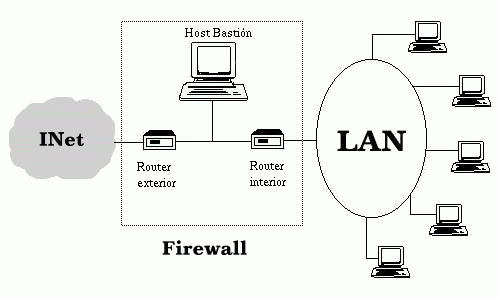
\includegraphics[width=\textwidth]{dmz.png}
\caption{Arquitectura DMZ.}
\label{dmz}
\end{center}
\end{figure}
\\Esta arquitectura de cortafuegos elimina los puntos \'unicos de fallo 
presentes en las anteriores: antes de llegar al basti\'on (por definici\'on, el
sistema m\'as vulnerable) un atacante ha de saltarse las medidas de seguridad 
impuestas por
el enrutador externo. Si lo consigue, como hemos aislado la m\'aquina basti\'on 
en una subred estamos reduciendo el impacto de un atacante que logre 
controlarlo, ya que antes de llegar a la red interna ha de comprometer 
tambi\'en al segundo {\it router}; en este caso extremo (si un pirata logra 
comprometer el segundo {\it router}), la arquitectura DMZ no es mejor que un 
{\it screened host}. Por supuesto, en cualquiera de los tres casos (compromiso
del {\it router} externo, del {\it host} basti\'on, o del {\it router} interno)
las actividades de un pirata pueden violar nuestra seguridad, pero de forma
parcial: por ejemplo, simplemente accediendo al primer enrutador puede aislar 
toda nuestra organizaci\'on del exterior, creando una negaci\'on de servicio 
importante, pero esto suele ser menos grave que si lograra acceso a la red
protegida.\\
\\Aunque, como hemos dicho antes, la arquitectura DMZ es la que mayores niveles
de seguridad puede proporcionar, no se trata de la panacea de los cortafuegos.
Evidentemente existen problemas relacionados con este modelo: por ejemplo, se 
puede utilizar el {\it firewall} para que los servicios fiables pasen 
directamente sin acceder al basti\'on, lo que puede dar lugar a un 
incumplimiento de la pol\'{\i}tica de la organizaci\'on. Un segundo problema,
quiz\'as m\'as grave, es que la mayor parte de la seguridad reside en los {\it
routers} utilizados; como hemos dicho antes las reglas de filtrado sobre 
estos elementos pueden ser complicadas de configurar y comprobar, lo que puede
dar lugar a errores que abran importantes brechas de seguridad en nuestro 
sistema.\\
\subsection{Otras arquitecturas}
Algo que puede incrementar en gran medida nuestra seguridad y al mismo tiempo
facilitar la administraci\'on de los cortafuegos es utilizar un basti\'on
diferente para cada protocolo o servicio en lugar de uno s\'olo; sin embargo,
esta arquitectura presenta el grave inconveniente de la cantidad de m\'aquinas
necesarias para implementar el {\it firewall}, lo que impide que muchas 
organizaciones la puedan adoptar. Una variante m\'as barata consistir\'{\i}a en
utilizar un \'unico basti\'on pero servidores {\it proxy} diferentes para
cada servicio ofertado.\\
\\Cada d\'{\i}a es m\'as habitual en todo tipo de organizaciones 
dividir su red en diferentes subredes; esto es especialmente aplicable en
entornos de I+D o empresas medianas, donde con frecuencia se han de conectar 
campus o sucursales separadas geogr\'aficamente, edificios o laboratorios 
diferentes, etc. En esta situaci\'on
es recomendable incrementar los niveles de seguridad de las zonas m\'as
comprometidas (por ejemplo, un servidor donde se almacenen expedientes o datos
administrativos del personal) insertando cortafuegos internos entre estas zonas
y el resto de la red. Aparte de incrementar la seguridad, {\it firewalls} 
internos son especialmente recomendables en zonas de la red desde la que no se
permite {\it a priori} la conexi\'on con Internet, como laboratorios de
pr\'acticas: un simple PC con Linux o FreeBSD que deniegue cualquier conexi\'on
con el exterior del campus va a ser suficiente para evitar que los usuarios 
se dediquen a conectar a p\'aginas {\it web} o {\it chats} desde equipos no
destinados a estos usos. Concretamente en el caso de redes de universidades 
ser\'{\i}a muy
interesante filtrar las conexiones a {\sc irc} o a {\sc mud}s, ya sea a nivel
de aulas o laboratorios o a nivel de todo el campus, denegando en el {\it 
router} de salida de la red hacia INet cualquier tr\'afico a los puertos 6667,
8888 y similares; aunque realmente esto no evitar\'{\i}a que todos los
usuarios siguieran jugando desde los equipos de la universidad -- por ejemplo 
a trav\'es de un servidor que disponga de conexi\'on en otros puertos --, 
s\'{\i} conseguir\'{\i}a que la mayor parte de ellos dejara de hacerlo.
